\chapter{RoFi Driver}\label{chap:software}

The RoFI platform does not give any restrictions on the implementation of
modules. However, having all the modules based on the same platform is an
advantage. Therefore, we consider implementation of universal module to be a
reference implementation of the other modules and we expect all the other
modules to reuse it as much as possibly. In this chapter we present several
tools and concepts designed for the implementation of the universal module.

We expect the firmware for modules to be developed using standard programming
means for the ESP32 microcontroller. That is the firmware is developed using C++
facilitated by the ESP-IDF \cite{noauthor_esp-idf_nodate} framework. The
framework provides drivers for MCU peripherals, FreeRTOS, the standard C and C++
libraries, and also offers several useful libraries (lwIP for network
communication, Bluetooth library or library for virtual file system). The
framework exposes its functionality as a plain C interface. In addition, many of
the provided functionality is also wrapped in POSIX-compatible interface. E.g,
sockets are accessible by both, lwIP interface and POSIX interface. The same
follows for threading; user can use FreeRTOS API or can leverage POSIX interface
or can even use C++ STL API.

The ESP32 provides sufficient tools for software development using stand modern
means. However, this means only cover general software development needs. We do
not want the user to write a custom library for controlling the motors, docks
and other. Therefore, we also provide \emph{RoFI Driver}, a software library
which provides interface to RoFI specific tasks.

The RoFi Driver consists of three parts: \todo{XXX}.

\section{The RoFI "BIOS"}

\section{Reactive Blocks Library}

Software development for robots and embedded systems is considered to be more
challenging than a classical software development. There are several reasons
why the development is challenging:
\begin{enumerate*}
    \item the microcontroller peripherals have to be mastered,
    \item testing and debugging is harder as the system is not self-contained a
    interacts with the environment, and
    \item the code has to deal with numerous asynchronous events and there task
    which needs to be distributed in time.
\end{enumerate*}

The challenge of mastering complicated peripherals can be mitigated by writing a
suitable high level drivers. Such drivers provide abstraction and hide
implementation on the hardware level. Therefore the user does not need to toggle
individual bits in configuration registers. Also the peripherals of modern
microcontrollers are more powerful and general and therefore, allow for good
abstraction. ESP-IDF provides such drivers for ESP32.

The burden of testing robotic software can be partially mitigated by splitting
the software into two layers -- the control layer operating on top an
input/output layer. The I/O layer interacts with peripherals drivers, interacts
with the environment and provide rather high level inputs to the control layer.
With setup it is possible to mock-up the I/O layer and perform standard software
testing of the control layer. However, testing is still rather challenging and
we do not bring any innovation in this field.

There are currently two classical approaches to tackle the burden of handling
asynchronous events in languages like C or C++. First, a real-time operating
system (RTOS) can be used with several tasks. Each task handles events in
synchronous, blocking, manner. This approach leads to a readable code as the
logic for handling events is kept close together and follows chronological flow
of the events. However, it might not preserve the lowest possible latency due to
RTOS task switching and also does not scale well as each the number of tasks is
usually limited. The second approach uses callback functions which are called to
handle an event. This approach scales well, however it leads to hard-to read
code as the callbacks do not preserve context and are spread all over the source
code. This phenomenon is usually referred as ``callback hell''. Also, code
complexity increases tremendously when error handling is added.

We designed a new solution for handling asynchronous events for the RoFI
platform. We call it \emph{reactive blocks}. The idea behind reactive blocks is
simple -- we use the same principle as callbacks, however, we provide a
syntactical sugar to write them in a chain-like structure to preserve the
chronological flow of event handling. Reactive blocks are inspired by the
ReactiveX library \cite{noauthor_reactivex_nodate} and the ranges-v3 library
\cite{noauthor_range-v3_nodate}.

The reactive blocks will be implemented as a stand-alone RoFi independent C++
library -- \emph{Ractive Blocks Library} (RBL). The library targets all
platforms with C++17 support and STL support. This includes standard variants of
x64, ARM and also embedded platform like ESP32 a or ARM COrtex-M. As the library
implementation is a subject of another thesis, we provide only a brief
description of its core functionality and omit some semantical nuances and the
implementation details.

Consider following (rather artificial) scenario: when a noisy distance sensor
overcomes a given threshold (generates edge), the robot notifies several other
robots (judges) over a network. The judges vote and if a majority votes yes, the
robot flashes a LED. For simplicity, consider a line-based text communication
protocol between the robots and numerous reasonably named functions.

Standard implementation using blocking interface might look like this:
\begin{minted}{cpp}
while ( true ) {
    // Wait rising edge debounced by 10 samples
    ring_buffer< int > samples( 10, 0 );
    while ( !all( samples,
                  []( int x ){ return x > threshold; } ) )
    {
        samples.push( sensor.read() );
        delay( 10_ms );
    }
    int sensorValue = average( samples );

    // Perform voting
    std::vector< bool > votes;
    for ( auto& judge : judges ) {
        judge.send( "value: " + std::to_string( sensorValue ) )
        vote = judge.receiveLine() == "yes";
        votes.push_back( vote );
    }

    // Flash an LED
    if ( majority( votes, []( bool vote ){ return vote; } ) ) {
        led.on();
        delay( 200_ms );
        led.off();
    }
}
\end{minted}

The sample code is straightforward and easily readable. By putting the code in a
separate task, we can handle multiple asynchronous events simultaneously.
However, the code does is not efficient as possible as the network communication
is synchronous.

Each asynchronous function traditionally takes a callback function as its
argument. The callback is called, when the operation is finished. The result
value or error is passed to the callback. The task from our example scenario
could be implemented like this using asynchronous interface:

\begin{minted}{cpp}
std::vector< bool > votes;
template < typename Callback >
void onJudgeResponse( const std::string& resp, Callback c ) {
    votes.push_back( resp == "yes" );
    if ( votes.size() == judges.size() &&
         majority( votes, []( bool vote ){ return vote; } ) )
    {
        c();
    }
}

template < typename Callback >
void vote( int value, Callback c ) {
    for ( auto& judge : judges ) {
        judge.send( "value: " + std::to_string( sensorValue ), [=] {
            judge.receiveLine( [=]( const std::string& s ) {
                onJudgeResponse( resp, s, c );
            } );
        } );
    }
}

ring_buffer< int > samples( 10, 0 );
timer.every( 10_ms. [&ring_buffer]() {
    samples.push( sensor.read() );
    if ( all( samples,
        []( int x ){ return x > threshold; } ) )
    {
        vote( average( samples ), judges, []{
            led.on();
            timer.after( 200_ms, []{
                led.off();
            });
        });
    }
});
\end{minted}

The code is now fully asynchronous, but is hard to read -- it does not preserve
the chronological order of event handling, the user have to think about shared
states and has a lot of nested sections. The need for a shared state arises from
the absence of information in the control flow of the program. E.g, the function
\texttt{onJudgeResponse} has to check if it is the last call of the function. In
the first example there is no such need as the the control captures the
information -- once the if-clause is reached, it is clear all judges voted.

The solution we provide is shown in code snippet below. We do not expect the
reader to immediately understand all details of the code as explanation
follows. We advise the reader to return to this example during the rest of
this section.

\begin{minted}{cpp}
auto overThreshold( std::pair< int, int > value ) {
    return value.first > threshold;
}

auto is( const std::string& what ) {
    return [=]( const std::string& s ) { return s == what; }
}

auto setLed( bool value ) {
    return [=]() { led.set( value ) };
}

auto sensorStream = timer.every( 20_ms ) >> sensor.read;
auto sensorAverage = sensorStream >> slidingAverage( 10 );
zip( sensorStream, sensorAverage)
    >> debounceOn( overThreshold )
    >> std::get< 1 >
    >> [&]( int sensorValue ) {
        return interleave( judges, [=]( auto& judge ) {
            std::string msg =
                "value: " + std::to_string( sensorValue );
            return judge.send( message )
                    >> judge.receiveLine >> is( "yes" );
        } ) >> majority;
    }
    >> setLed( true ) >> wait( 200_ms ) >> setLed( false );
\end{minted}

The reactive blocks follow similar idea as the range-v3 library -- we describe a
pipeline for data transformation, however unlike ranges-v3, the data might be
scattered over time. By describing the pipeline the user can preserve
chronological ordering of the event handling in the code but also preserves
asynchronicity at the same time. In the traditional future concept, which also
allows to describe a pipeline, the pipeline is only linear and allows only a
single value to pass. The reactive blocks allow for non-linear pipelines and
also allows multiple values to pass through it. Visualization of the pipeline
for the example above is shown in figure \ref{fig:rbl_example_1}.

\begin{figure}[!t]
    \centering
    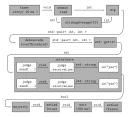
\includegraphics[]{figures/rbl_pipeline_1.pdf}
    \caption{Pipeline visualization for sensor and voting code snippet.}
    \label{fig:rbl_example_1}
\end{figure}

Reactive blocks allow to chain data transformation operations -- just like UNIX
pipe operator. Each operation is represented by a block. There are two type of
blocks: \mintinline[breaklines]{cpp}{template < typename T > Puslisher< T > }
and \mintinline[breaklines]{cpp}{template < typename T > Subscriber< T > }.
Single block can be both publisher and subscriber.

\noindent The publisher can:
\begin{enumerate}
    \item emit an arbitrary number of values of type \texttt{T} at any time (we
    say it generates a \emph{stream} of values),
    \item emit an error (object inheriting from
    \mintinline[breaklines]{cpp}{std::exception}), and
    \item close itself (mark the end of its stream). After closing no more
    values nor errors can be emitted.
\end{enumerate}

\noindent The subscriber can subscribe to a to publisher. After subscribing it
\begin{enumerate}
    \item receives values of type \texttt{T} emitted by the publisher and
    \item can unsubscribe.
\end{enumerate}

The simplified implementation of subscriber and publisher is provided in the
following snipped. Note that the implementation omit all technical aspects like
management of object life-time and only shows the bare minimum of functionality.
\begin{minted}{cpp}
template < typename T >
class Publisher {
public:
    void subscribe( Subscriber< T >* s ) {
        _subscribers.push_back( s );
    }
    void unsubscribe( Subscriber< T >* s ) {
        _subscribers.erase(
            std::remove( _subscribers.begin(),
            _subscribers.end(), s ), _subscribers.end() );
    }
protected:
    void publish( T t ) {
        for ( auto& s : _subscribers )  s->onvalue( t );
    }

    void publishError( const std::exception& e ) {
        for ( auto& s : _subscribers )  s->onError( e );
    }

    void close() {
        for ( auto& s : _subscribers )  s->onClose();
    }
private:
    std::vector< Subscriber< T >* > _subscribers;
};

template < typename T >
class Subscriber {
protected:
    virtual void onValue( T t ) = 0;
    virtual void onError( const std::exception& e ) = 0;
    virtual void onClose() = 0;
};
\end{minted}

With these base classes we can derive any other reactive block. For example we
can build a block which converts a number to string:
\begin{minted}{cpp}
class N2S: public Publisher< std::string >,
    public Subscriber< int >
{
    virtual void onValue( int i ) override {
        publish( std::to_string( i ) );
    }
    virtual void onError( const std::exception& e ) override {
        publishError( e );
    }
    virtual void onClose() override {
        close();
    }
};
\end{minted}

Or, given a classical callback-based asynchronous interface in form of function
\mintinline[breaklines]{cpp}{errorCode asyncFoo( int param, Callback c )} we can
wrap it inside a block which accepts the input for the asynchronous function and
produces the output.
\begin{minted}{cpp}
class AsyncFoo: public Publisher< int >,
    public Subscriber< int >
{
    virtual void onValue( int i ) override {
        errorCode = asyncFoo( i, [&]( int retval ) {
            this->publish( retval );
        } );
        if ( errorCode == ERROR )
            publishError(
                std::runtime_exception( "Something wrong" ) );
    }
    virtual void onError( const std::exception& e ) override {
        publishError( e );
    }
    virtual void onClose() override {
        close();
    }
};
\end{minted}

In similar manner all asynchronous events can be wrapped inside a reactive block
-- including interrupts or possibly, but not preferably, busy waiting. Note,
that the reactive blocks does not bring asynchonicity in the system, they just
provide a new interface for it. The blocks can also wrap synchronous tasks as
shown in the example of the \texttt{N2S} class. The only requirement is that the
code inside a block should not block for a long time as it might delay other
pending blocks. Also, there can be $m$-to-$n$ mapping of incoming values to the
block, not just 1:1 mapping as we showed in the examples. The block can emit
multiple values from a single input value (e.g., block splitting string
according to a delimiter or timer producing values at a given period).

When multiple block are linked together via the subscribe relation, we call the
final structure chain. Therefore, we will refer to the operation as
\emph{chaining blocks}. Chains are first-class citizens just like blocks.
Therefore we can store them in variable or chain multiple chains together.

However, building the block manually by defining classes is verbose and leads to
hard-to-read code. Therefore, the library provides operator
\mintinline[breaklines]{cpp}{>>} (chain). The operator is similar to Haskell's
bind operator -- it build the subscribe relation between chains. The operator
comes in many overloads and provides implicit creation of blocks out of
functions. This functionality provides a syntactical sugar, which allows to make
the code less verbose and also allows to keep the code in a chronological order.

To further simplify the code, the library should provide predefined blocks like:
zip (takes two stream of values and combines them together in pairs), interleave
which takes multiple streams and joins them together, simple waiting, etc.

The last advantage of reactive blocks we present is error handling. The
publishers can publish value or an error. By default, the error goes through the
pipeline until some block stops it and handles it. This provides a monadic- and
exception-like behavior. See following example:
\begin{minted}{cpp}
a >> b >> c >> onError( []( std::exception& e ) {
    std::cerr "Error a-c: " << e.what() << std::endl();
} ) >> d >> e >> onError( []( std::exception& e ) {
    std::cerr "Error d-e: " << e.what() << std::endl();
} );
\end{minted}
The code defines a linear chain of blocks \texttt{a} to \texttt{e}. If any of
the block fails, the error is captured by one the two error handlers. Also, the
chain operator by default captures exception thrown out of functions and sends
them down the chain:
\begin{minted}{cpp}
a >> [] {
    throw std::runtime_error( "Inevidable error" );
} >> b >> onError( []( std::exception& e ) {
    std::cerr "Inevidable error follows:  "
        << e.what() << std::endl();
} );
\end{minted}

In the text above, we presented the library using a runtime polymorphism, which
might not be suitable for embedded platforms. However, for chains with a type
known in the compile time the runtime polymorphism could be eliminated in the
future releases of the library. The runtime polymorphism elimination also allow
for further optimization and reducing the cost of the reactive blocks
abstraction.

\section{RoFI Driver Interface}

\section{Remote Procedure Call}